\documentclass{article}

\usepackage[normalem]{ulem}
\usepackage{fancyhdr}
\usepackage[parfill]{parskip}
\usepackage{tikz}
\usepackage{pgfplots}
\usepackage{multicol}
\usepackage{mhchem}
\pagestyle{fancyplain}

\title{Atomic structure}
\author{Todd Davies\\
	\texttt{\small todd434@gmail.com}}
\date{\today}

\begin{document}

\rhead{Atomic structure}
\lhead{\today}

\maketitle

\section*{Alpha particle scattering and the nucleus}
\thispagestyle{empty}

\section*{The simple atomic model}

\section*{Nucleons and electrons}

An atom can be described by the particles that it contains. The basic set of
particles that define atoms are well known, and are as follows:

\begin{center}
\begin{tabular}{l|l|l}
	{\bf Particle} & {\bf Relative mass} & {\bf Charge} \\ \hline
	Proton & 1 & +{\it e}\\ \hline
	Neutron & 1 & 0\\ \hline
	Electron & $\frac{1}{1836}$ & -{\it e}
\end{tabular}
\end{center}

\textit{N.b. Protons and neutrons are often refered to as Nucleons, since they
usually reside in the nucleus of atoms.}

\subsection*{Nuclear notation}

There is a specific notation for writing down what an atom is composed of, it
looks like this:

\[
	\ce{^{\textrm{\it Nucleon number }}_{\textrm{\it Proton number }} X}
\]

\subsection*{Isotopes}

An isotope of an element contains a different number of {\it neutrons} to the
element. This means that it's mass is different and the nucleus of the atom is
potentially unstable. However, it still has the same amount of electrons in it's
outer energy level, so the interactions between it and other atoms are the same.

\section*{Forces in the nucleus}

It is suprising that the nucleus doesn't blow apart, since it is made up of
positive and neutral particles and no negative particles. However, there are
more forces at work inside the nucleus that mean it doesn't just fall apart as
expected.

The force that counteracts the electrostatic forces in the nucleus is called the
{\it strong force}. It only acts over very short distances ($10^{-14}m$) and the
magnitude of the force is related to the seperation between the nucleons.

This graph shows how the strong force changes with distance:

\begin{center}
	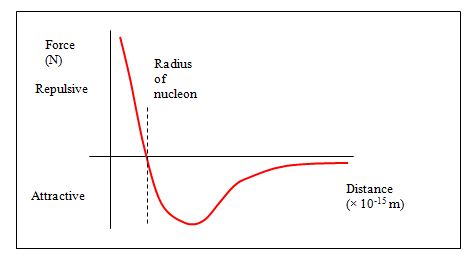
\includegraphics{strong_force_graph}
\end{center}

\subsection*{Padding with neutrons}

The strong force still doesn't explain why neutrons are present in the nucleus.
The strong force should act between the protons to keep them bound together,
yes?

In actual fact, the strong force acts only once between each pair of protons
(since it only acts over a distance equal to the radius of a proton). On the
other hand, electrostatic attraction acts over a large distance, so each proton
doesn't just repel the proton next to it, but also repells all of the protons
that it is near to. The combined electrostatic repulsions are greater than the
strong force.

This explains why neutrons are present in the atom. They increase the distance
between the protons so the electrostatic repulsion between them is reduced, yet
they are also affected by the strong force. This has the effect of balancing the
force in the atom and stableising the nucleus. This is also why isotopes with
the incorrect number of neutrons are usually unstable.

\section*{Families of particles}
There are two classes of sub-atomic particles that we use, leptons and hadrons.

\subsection*{Leptons}

Particles that are unaffected by the strong force are leptons. There are twelve
leptons altogether, since each of the 'main' three (the electron, the muon and
the tau) has an associated neutrino and they all have antiparticles.


\end{document}